\documentclass[12pt]{article}
\usepackage[margin=1.5cm]{geometry}
\usepackage{parskip}
\usepackage{amsmath}
\usepackage{amssymb}
\usepackage{amsfonts}
\usepackage{enumitem}
\usepackage{graphicx}
\usepackage{stmaryrd}
\graphicspath{ {./images/} }


\begin{document}
\begin{enumerate}[label=(\alph*)]
  \item
    \begin{enumerate}[label=(\roman*)]
      \item
        The motivation behind phylogenetics is to be able to create some kind of evolutionary tree from just the DNA sequences of different species. This allows biologists to get an idea of how closely related different species are, and what their common ancestors might be.

      \item
        One technique for phylogeny is the UPGMA algorithm. The UPGMA algorithm takes as input some distance metrics between sets of species (e.g. from pairwise alignments).

        This algorithm works by progressively clustering species. We start with each species in its own cluster, and then iteratively join together the two closest clusters (based on average distance), until we are left with just a single cluster.

        For example, suppose we are clustering three species $A$, $B$, $C$, with $A$ and $B$ having a distance of 1, and $C$ having a distance of 10 from $A$ and $B$, we get the following tree:

        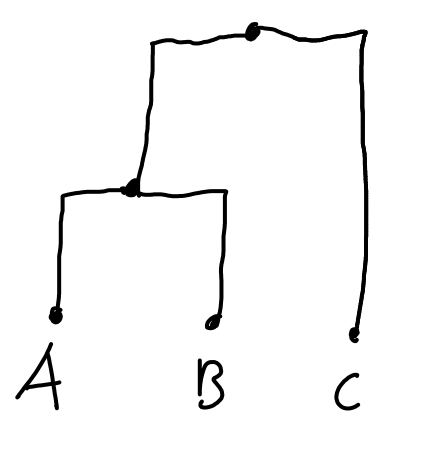
\includegraphics[scale=0.3]{upgma}

        UPGMA has time complexity $O(n^2)$ with $n$ species, which is relatively fast, but comes at the expense of being quite crude.


        \vspace{20pt}

        Another technique for phylogeny is Sankoff's algorithm for small parsimony. This is a parsimony-based technique, as opposed to a distance-based technique like UPGMA, so we hope that we are able to create a better algorithm by taking into account the actual DNA sequences themselves, and not just using proxy metrics like distance.

        This algorithm takes as input an unrooted tree, where the leaves are labelled with a DNA sequence. Then, character by character, we label the internal nodes of the tree based on the fewest state changes required to get there, using a dynamic programming algorithm, and the score of the tree is the sum of the state changes we needed, which we want to minimise.

        For example, we could use the algorithm as follows:

        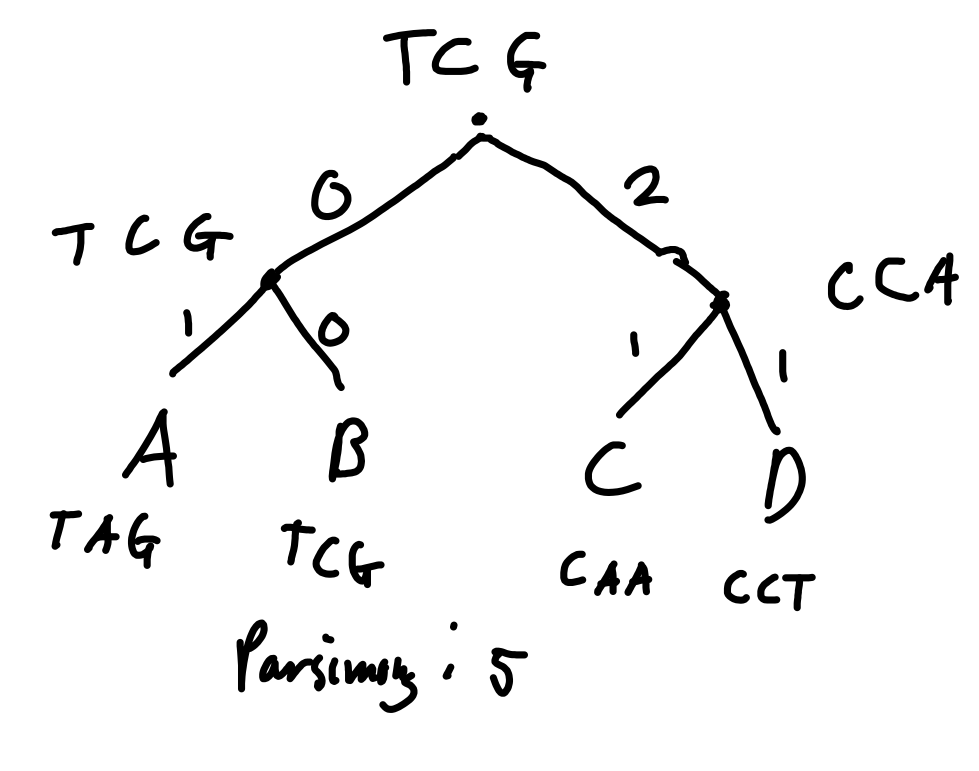
\includegraphics[scale=0.3]{parsimony}

        This algorithm provides labellings of internal nodes, but does require us to design a tree structure ourselves, so is somewhat limited on its own, and has complexity $O(mnk^2)$, if there are $n$ species with DNA sequences of length $n$ with $k$ internal states of the tree, which is much larger than the $O(n^2)$ we had for UPGMA.

    \end{enumerate}

  \item
    \begin{enumerate}[label=(\roman*)]
      \item
        In such a hidden Markov model, we first need to decide on a representation of hidden states and emissions. In our case, the membrane segment types (e.g. in membrane, out of membrane, etc.) would be the hidden states, and the emissions would be the amino acids.

        Then, we need our emission and transition probability matrices, which we might decide upon through biological reasoning, or by frequency from some ground truth data.

        Given an amino acid sequence, we then need to predict the what parts of the sequence correspond to which membrane type, i.e. finding the hidden states given the emissions. This process is called decoding, and can be solved using the Viterbi algorithm.

        The Viterbi algorithm is a dynamic programming algorithm that considers, at each subsequent time-step/position, what is the probability of each state, given the emission we are seeing, and the probabilities of each of the previous states (assuming a first-order model here). Then, once this matrix of probabilities is computed, we can compute the most likely state path by backtracking from the end, which gives us our predicted sequence of hidden states/membrane segments.

      \item
        The sensitivity and specificity of an HMM correspond to the true positive rate and the true negative rate respectively.

        Given an HMM, we can assess its performance if we apply it to some data for which the truth is already known, e.g. in the example from (b)(i), the types and locations of each of the membrane segments compared to the amino acid sequence.

        Then, for each of the predicted states, we can determine whether the HMM correctly predicted positive/negative (assuming we divide our states into two categories, like in-membrane and out-membrane).

        We can count up all of the times the underlying data was actually positive, and divide that by the number of times the HMM correctly predicted the state was positive, which gives us our TPR/sensitivity. 

        We can count up all of the times the underlying data was actually negative, and divide that by the number of times the HMM correctly predicted the state was negative, which gives us our TNR/specificity.
        
    \end{enumerate}
        
\end{enumerate}
\end{document}
